% status: 100%
% chapter: TBD

\title{Power BI}

\author{Surya Prakash Sekar}
\affiliation{%
  \institution{Indiana University
  Bloomington} \city{Bloomington} \state{Indiana} \postcode{47408} \country{USA}
  }
\email{sursekar@iu.edu}

% The default list of authors is too long for headers}
\renewcommand{\shortauthors}{Surya Prakash Sekar}

\begin{abstract}
Power BI is a business analytics tool offered by Microsoft. It is mainly used 
in the industry for analyzing data, creating interactive dashboards for 
visualization, business intelligence features and its wide range of cloud 
services. It is notable for its ability to connect with a wide range of data 
sources on the cloud, data preparation capabilities and extracting business 
insights from the data. It has many advanced features which is really helpful 
in the industry in terms of creating secure and advance dashboard visualizations.
\end{abstract}

\keywords{hid-sp18-418, visuals, data model, cloud-services, Business Insights}
%use up to 5 keywords

\maketitle

\section{History}
Power BI was launched by Microsoft in September 2013 as Power BI for 
Office 365. The initial release of Power BI was based on the Microsoft 
Excel–based add-ins like Power Query, Power Pivot and Power View. Microsoft kept 
adding many additional features like Question and Answers, enterprise level 
data connectivity and security options via Power BI Gateways throughout time. 
Power BI was first released to the public on July 2015
~\cite{hid-sp18-418-powerbi-history}.

\section{Introduction}
Power BI facilitates the creation of interactive visualizations, reports and 
dashboards that are shared across the cloud, also features to type 
natural-language questions about the data on the dashboard, handling files 
that are too large for Excel are available in it
~\cite{hid-sp18-418-powerbi-intro}.
Power BI includes both a desktop program and a cloud service. The cloud service 
is multi-platform which runs on Microsoft Edge, Internet Explorer, Chrome, 
Safari for Mac and Firefox. There are also mobile apps for iOS, Android and 
Windows that enables viewing of the Power BI or SQL Server Reporting Services 
reports and dashboards in devices like mobile phones and tablets.

\section{Terminologies}

\subsection{Power Query}
Power Query is an Excel add-in that can be used for data 
discovery, data reshaping and aggregating the data from various sources. 
Power Query is one of the Excel add-ins provided as part of Microsoft Power 
BI self-service solution~\cite{hid-sp18-418-powerbi-intro}.

\subsection{DAX}
Data Analysis Expression, is a formula language. DAX is used to define 
custom calculations for calculated columns and measures. DAX includes some of 
the formulas used in excel~\cite{hid-sp18-418-dax-basics}.

\subsection{Content Pack}
Content Pack is a collection of predefined visualizations and reports 
with respect to certain sample data sources.

\subsection{Quick Insights}
Quick Insights is a functionality within Power BI which enables it to 
deep dive into the connected dataset for hidden insights and display certain generated 
visuals with respect to any dataset accordingly.

\subsection{PowerPivot}
PowerPivot uses an in-memory engine called VertiPaq. 
This SSAS engine takes advantage of the increased RAM available in the 
PC thus enabling the calculations and the aggregations to be comparatively 
faster, it works on DAX~\cite{hid-sp18-418-powerpivot}.

\subsection{Power View}
Power View is a data visualization technology that allows the 
creation of interactive charts, graphs, maps, and other visuals which is 
very effective in Ad hoc analysis.

\subsection{R-Powered Visuals}
R code can be written to construct visualizations using Power BI.

\section{Components}

\subsection{Power BI Desktop}
Power BI Desktop is mainly used to create reports and data visualizations on
the dataset, it is a desktop-based application. Power BI Desktop can also be used to 
build data models and the dashboards can be shared by publishing it to the Power BI service. 
Also, it is available for free to download online.

\subsection{Power BI Gateway}
Power BI on-premises gateway is used to keep the data fresh 
by connecting to on-premise data sources without needing to move the data. It 
enables querying large datasets and benefiting from the existing investments
~\cite{hid-sp18-418-powerbi-components}.

\subsection{Power BI Mobile Apps}
Power BI mobile apps can be used to view the dashboards and the data in mobile 
phones. Power BI apps are available across Windows, iOS, and Android platform. 
The dashboards are automatically rescaled with respect to our devices.

\subsection{Power BI Service}
Power BI Service is a cloud service and is mainly used to publish the 
Power BI reports and data visualizations on the cloud. Every dashboard hosted 
here is well secured because we would need to authenticate via email by providing 
the email of our desired audience while sharing our work and only they would receive the 
link of the dashboard to view it. Microsoft also covered the security loophole involving exposure 
of the link to a dashboard to unauthorized personnel by granting viewership only to 
authenticated audience as directed by the author of the dashboard.
~\cite{hid-sp18-418-powerbi-components}.

\subsection{Power BI Embedded}
Power BI REST API can be used to build dashboards and 
reports into the custom applications that serves Power BI users
~\cite{hid-sp18-418-powerbi-components}. It could also be used for non-Power 
BI users as well.

\section{Installation}
We need a work or university email id in order to download Power BI Desktop. The basic 
version of Power BI with cloud service is available for free which offers 
1GB data storage which can be expanded through a paid account. Also, it extends
its automated data refresh, increased streaming capacity features to the paid 
accounts and it is not available in this basic version of Power BI. 
The published dashboards will be available on the cloud and can be accessed from 
the applications website of Power BI provided the individual has the access rights to the 
dashboard.
 
\section{Key Features}
Power BI desktop additionally offers basic data wrangling capabilities like Power Query 
from Excel. It can work with some unique data types like Salesforce, Google Analytics, 
MailChimp, GitHub, QuickBooks online and pull them from the cloud~\cite{hid-sp18-418-powerbi-intro}.
It has the capability to run R script files as well, indicating that any data 
that could be extracted by R can be imported into Power BI as well. 
Organizations can create their own content packs for getting data from their 
on-premise systems and the cloud services they use. What the content packs do 
is give Power BI the data model of the services it gets data from, so it can 
automatically build dashboards and charts to expose useful data, and so you 
can use the natural language Q and A feature. Power Q and A  is a natural language 
engine for the data model that we create in Power BI. Users can ask questions 
and answers would be processed and output with respect to the data model.Once 
the data model has been deployed into the Power BI website, then users can ask 
questions and get answers on the model~\cite{hid-sp18-418-powerbi-intro}. The 
Performance of the of Q and A is also quite remarkable and accurate.
The author of the dashboard can grant different types of access with respect 
to the hierarchy of the viewer based on the row level security concept within 
Power BI, which restricts data access depending upon the user.

 
\section{Dashboard Sample}
A toy dashboard using quick insights on Power BI using the sample Human 
Resource data available on it has been created below~\cite{hid-sp18-418-powerbi-sample-dataset}.
The dashboard and the report analyses the new hires, active employees and employees 
who quit to discover trends and insights with respect to the hiring strategy. The 
dashboard can be published online and in order to share it with a another personnel 
we would need to authorize by providing an email to the Power BI share module so that 
it can send the link of the dashboard to our desired audience and they would require 
a Power BI account as well to view the dashboard. The dashboard provides information 
regarding the bad hires, active employees and new hires of a firm with respect to various 
metrics. The visualization is generated by the quick insights feature of Power BI, 
which is capable of generating automated visualization with respect to a given dataset.

\begin{figure}[!ht]
\centering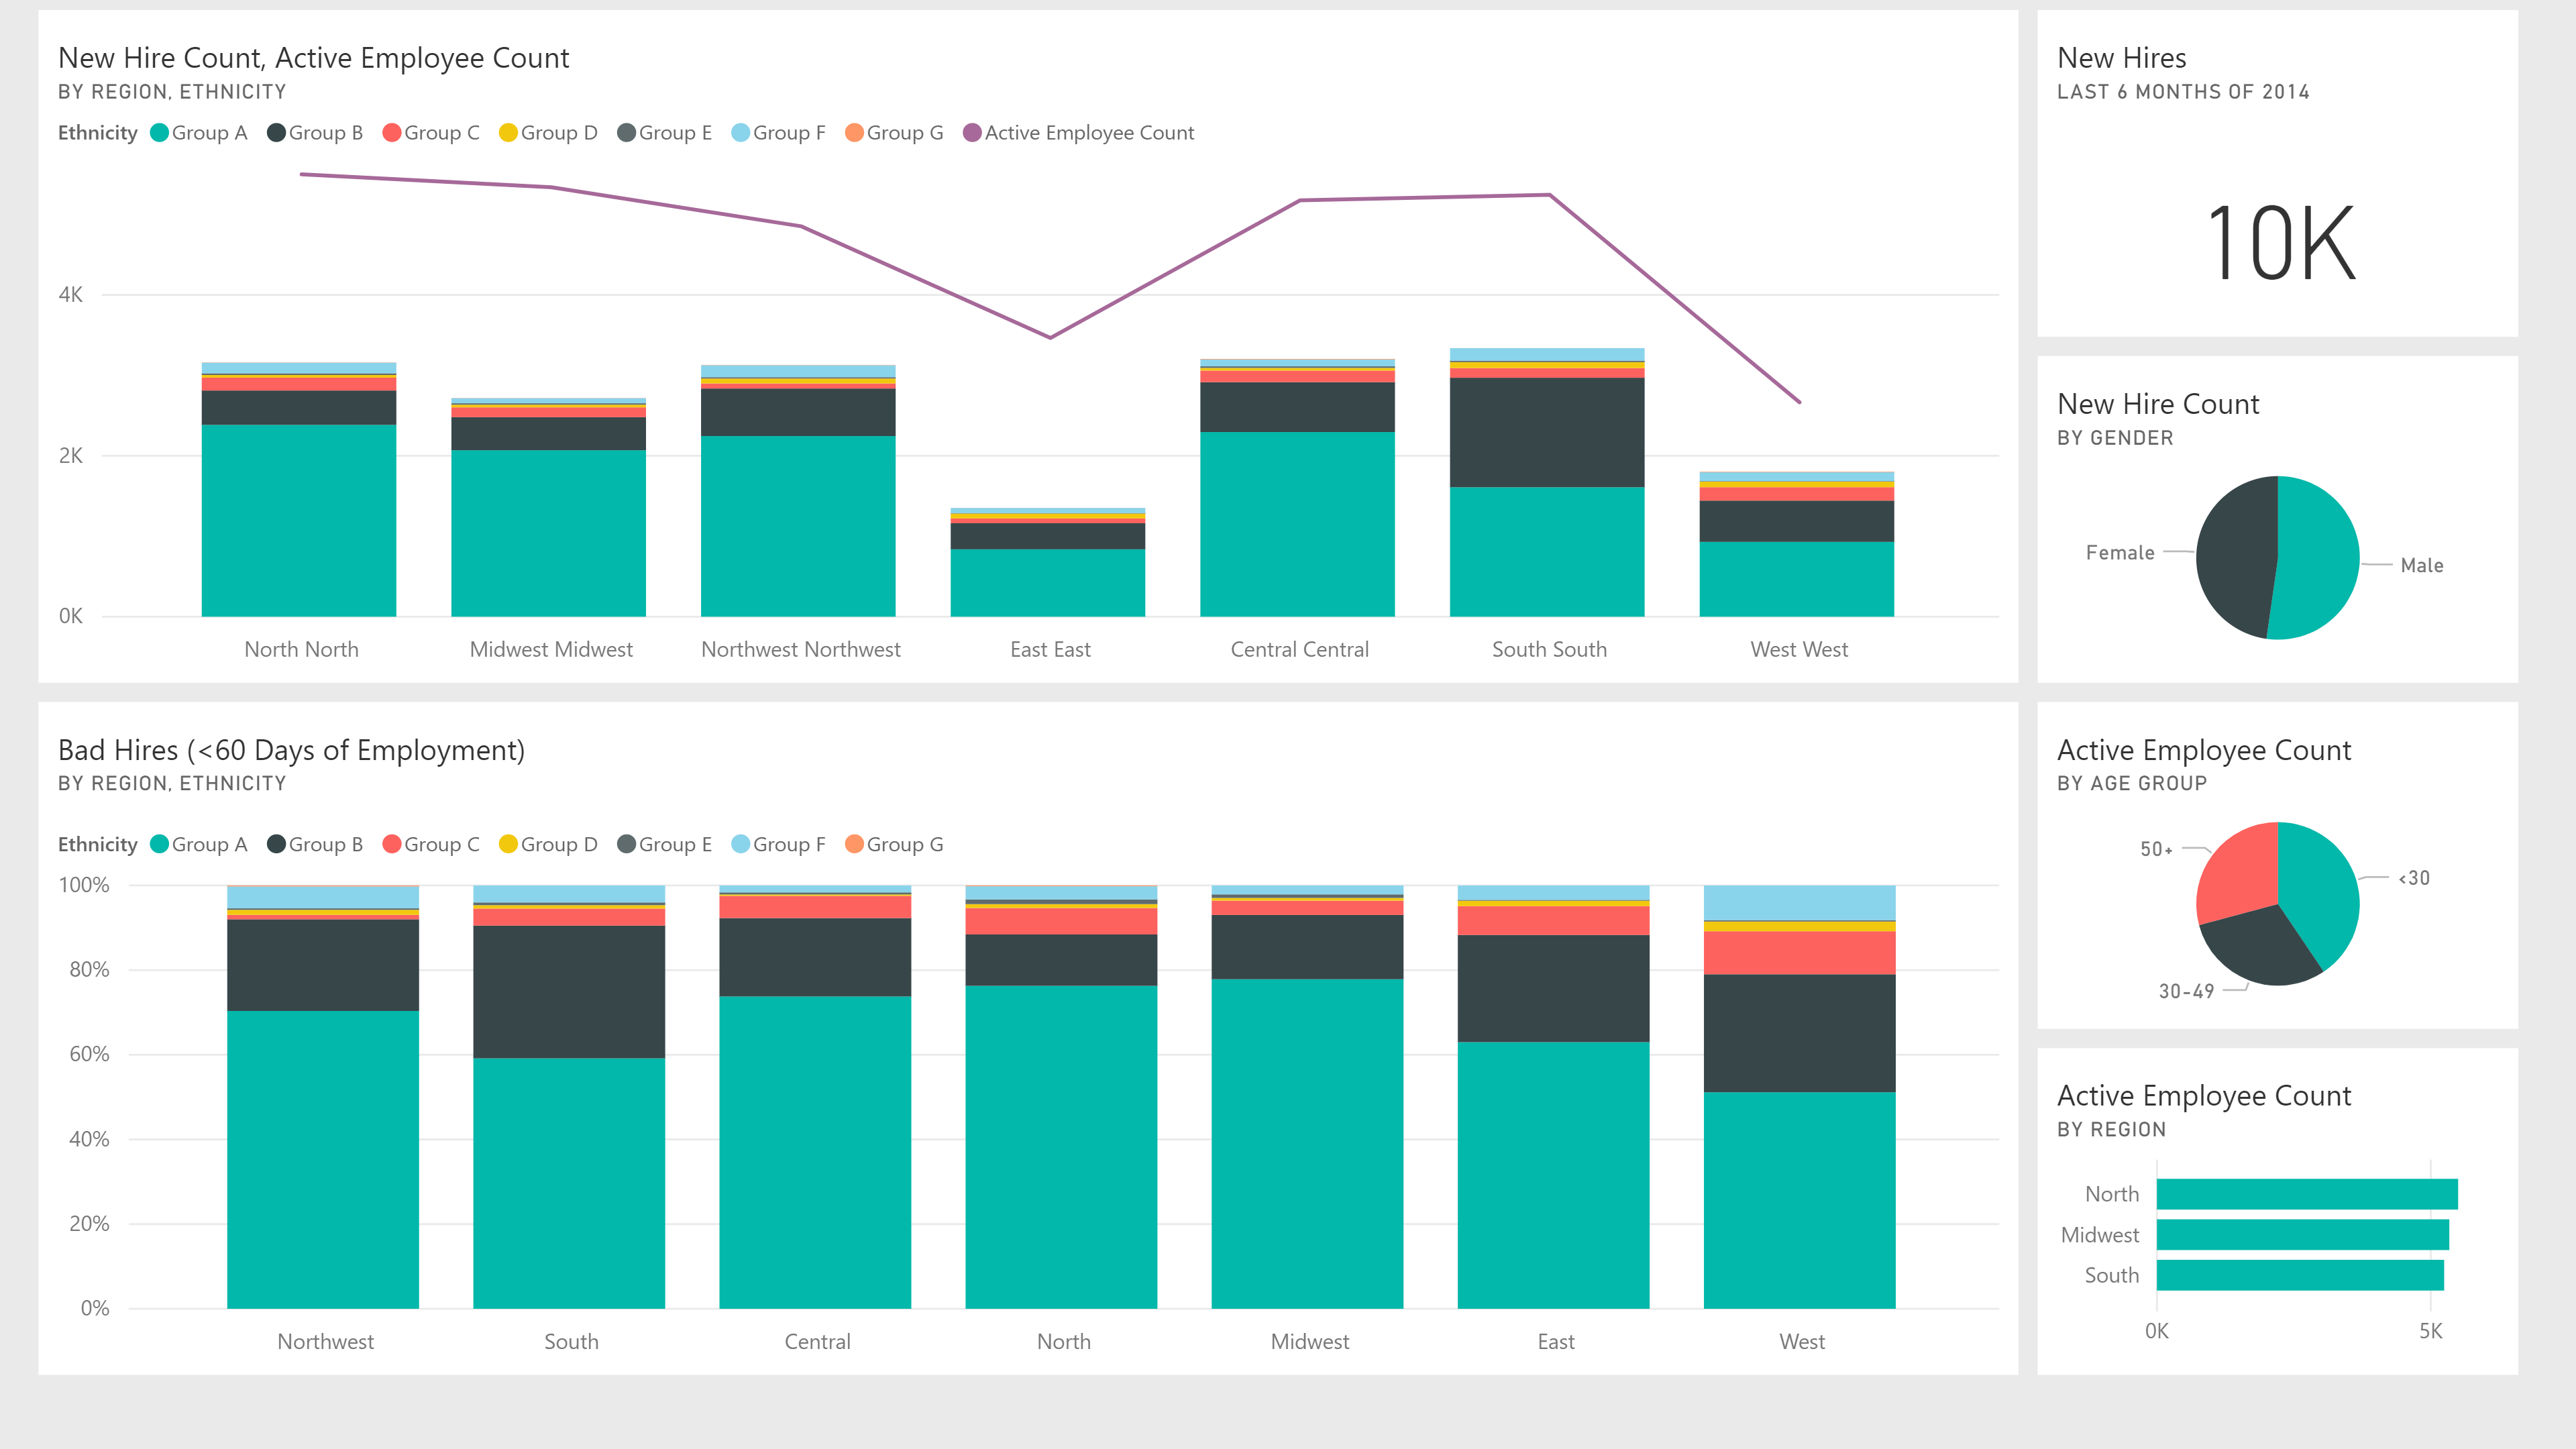
\includegraphics[width=\columnwidth]{../images/dashboard.png}
\caption{Sample Dashboard~\cite{hid-sp18-418-powerbi-sample-dashboard}}
\label{f:Dashboard}
\end{figure}

\section{Shortcomings}
Although Power BI has many advanced features with respect to the business intelligence 
domain, interactive visualizations, cloud features and data analysis. It does possess 
some flaws in comparison to its fellow competitors like tableau. 
\begin{enumerate}
\item \textbf{Handling big datasets:} When it comes to working with big datasets,
importing and connecting them would hurt the performance and cause timeouts~\cite{hid-sp18-418-powerbi-review}.
Hence third party tools like SQL Server is being used to overcome this shortcoming.
\item \textbf{Modularity:} There are many modules being released by Microsoft with 
respect to Power BI which is a positive in a way but,it leads to confusion with respect 
to the end user on what modules they require for a particular project as the list is 
really big and also since the number of modules increase the possibility of a module 
breaking is also respectively high~\cite{hid-sp18-418-powerbi-review}.
\item \textbf{Preprocessing:} Most visualization tools have some preprocessing modules 
installed within them which can be used to clean the data. But Power BI assumes that the 
data it deals with is already preprocessed, therefore the end user has to rely on other 
tools for preprocessing~\cite{hid-sp18-418-powerbi-review}. 
\item \textbf{Sharing:} In some cases sharing dashboards to public would be required, 
but it is not allowed in Power BI, we would need to authorize an email access to the audience 
of the dashboard. But, we can still share the reports of the dashboard to anyone with 
the help of a link.
\item \textbf{Learning:} One huge pitfall when it comes to Power BI is its complexity, 
since most of the end users would be from a variety of backgrounds mastering Power BI 
would take some significant amount of time in order to use its features efficiently. 
Whereas less complex tools in the industry offering similar features are easy to use 
even by non technical personnel.
\end{enumerate}

\section{Comparison with competitors}
Power BI is still emerging in the analytics industry and is actually making significant 
progress with respect to it competitors.

\subsection{Tableau}
In comparison to Power BI, Tableau is still ahead in the industry for creating and 
maintaining real time dashboards with integration to the data available in real time, 
but still Power BI provides similar features and also additional automated dashboard
refresh features in real time to stay in the competition~\cite{hid-sp18-418-powerbi-comparison}. 
Both the tools offer well sophisticated visualizations, charts and drill downs when 
it comes to dashboards. But in terms of ease of use and learning Tableau is still 
leading over all of its competitors and Power BI in terms of ease of use and learning 
is a bit complex comparatively. Power BI has complex features like Power Q and A, quick 
insigths and so on which tableau lacks although it has drag and drop visuals it is 
not as informative as Power BI. Finally, when it comes to sharing or publishing the 
work Tableau has an edge over Power BI because of its extended features and also, 
Power BI has its own restrictions in this area but at the same time making sure that 
the accessibility of the work is more secure.   

\subsection{Qlikview}
When comparing Power BI with respect to Qlikview, one huge downfall of Power BI 
lies in its data management capabilities, like mentioned previously Power BI relies 
more on third parties for it, whereas Qlikview has its own ETL~\cite{hid-sp18-418-powerbi-comparison}. 
Again when it concerns aspects like sharing and publishing Qlikview is better than 
Power BI due its restrictions as mentioned previously and also it is supported by 
many solutions. Qlikview is comapratively more adapatable than Power BI. 
There is feature in Qlikview called Finally, when it comes down to analyzing the 
entire platform, Power BI is built on a much more integrated and sophisticated 
platform making it better supportive than Qlikview in the industry ~\cite{hid-sp18-418-powerbi-comparison}.

\section{Conclusion}
Power BI in overall is being used as a cloud-based analytics environment which 
can be employed to solve a wide range of problems related to business analysis 
and automated cutting edge data visualizations. The extravagant features 
available offers Power BI an edge over its fellow competitors like Tableau, 
Qlikview and so on. The options to automate most of the operations makes 
Power BI the go to platform when it comes to building data models and sharing 
dashboards on the cloud in the industry. Having mentioned that there is still scope
for improvement in areas like data management, ease of use, publishing and sharing 
which would make Power BI a leader in its domain.
 
\begin{acks}

The authors would like to thank Dr.~Gregor~von~Laszewski for his
support and suggestions to write this paper.

\end{acks}

\bibliographystyle{ACM-Reference-Format}
\bibliography{report} 